\documentclass[dvipsnames,pdf, unicode, 12pt, a4paper, oneside, fleqn]{article}
\usepackage[utf8]{inputenc}
\usepackage[T2B]{fontenc}
\usepackage[english,russian]{babel}

\usepackage{listings}
\usepackage{longtable}
\oddsidemargin=-0.4mm
\textwidth=160mm
\topmargin=4.6mm
\textheight=210mm
\usepackage{geometry}
%% Страницы диссертациия должны иметь следующие поля:
%% левое --- 25 мм, правое --- 10 мм, верхнее --- 20 мм, нижнее --- 20 мм.
%% Абзацный отступ должен быть одинаковым по всему тексту и равен пяти знакам.
\geometry{
 a4paper,
 total={170mm,257mm},
 right=10mm,
 left=10mm,
 top=20mm,
 bottom=20mm,
}
\pagenumbering{gobble}






%Define the listing package
\usepackage{listings} %code highlighter
\usepackage{color} %use color
\definecolor{mygreen}{rgb}{0,0.6,0}
\definecolor{mygray}{rgb}{0.5,0.5,0.5}
\definecolor{mymauve}{rgb}{0.58,0,0.82}
 
%Customize a bit the look
\lstset{ %
backgroundcolor=\color{white}, % choose the background color; you must add \usepackage{color} or \usepackage{xcolor}
basicstyle=\footnotesize, % the size of the fonts that are used for the code
breakatwhitespace=false, % sets if automatic breaks should only happen at whitespace
breaklines=true, % sets automatic line breaking
captionpos=b, % sets the caption-position to bottom
commentstyle=\color{mygreen}, % comment style
deletekeywords={...}, % if you want to delete keywords from the given language
escapeinside={\%*}{*)}, % if you want to add LaTeX within your code
extendedchars=true, % lets you use non-ASCII characters; for 8-bits encodings only, does not work with UTF-8
frame=single, % adds a frame around the code
keepspaces=true, % keeps spaces in text, useful for keeping indentation of code (possibly needs columns=flexible)
keywordstyle=\color{blue}, % keyword style
% language=Octave, % the language of the code
morekeywords={*,...}, % if you want to add more keywords to the set
numbers=left, % where to put the line-numbers; possible values are (none, left, right)
numbersep=5pt, % how far the line-numbers are from the code
numberstyle=\tiny\color{mygray}, % the style that is used for the line-numbers
rulecolor=\color{black}, % if not set, the frame-color may be changed on line-breaks within not-black text (e.g. comments (green here))
showspaces=false, % show spaces everywhere adding particular underscores; it overrides 'showstringspaces'
showstringspaces=false, % underline spaces within strings only
showtabs=false, % show tabs within strings adding particular underscores
stepnumber=1, % the step between two line-numbers. If it's 1, each line will be numbered
stringstyle=\color{mymauve}, % string literal style
tabsize=2, % sets default tabsize to 2 spaces
title=\lstname % show the filename of files included with \lstinputlisting; also try caption instead of title
}
%END of listing package%
 
\definecolor{darkgray}{rgb}{.4,.4,.4}
\definecolor{purple}{rgb}{0.65, 0.12, 0.82}
 
%define Javascript language
\lstdefinelanguage{JavaScript}{
keywords={typeof, new, true, false, catch, function, return, null, catch, switch, var, if, in, while, do, else, case, break},
keywordstyle=\color{blue}\bfseries,
ndkeywords={class, export, boolean, throw, implements, import, this},
ndkeywordstyle=\color{darkgray}\bfseries,
identifierstyle=\color{black},
sensitive=false,
comment=[l]{//},
morecomment=[s]{/*}{*/},
commentstyle=\color{purple}\ttfamily,
stringstyle=\color{red}\ttfamily,
morestring=[b]',
morestring=[b]"
}
 
\lstset{
language=JavaScript,
extendedchars=true,
basicstyle=\footnotesize\ttfamily,
showstringspaces=false,
showspaces=false,
numbers=left,
numberstyle=\footnotesize,
numbersep=9pt,
tabsize=2,
breaklines=true,
showtabs=false,
captionpos=b
}







\usepackage{multicol}
\usepackage[]{amsmath}
\usepackage{multirow}

\usepackage{graphicx}
\graphicspath{{pictures/}}
\DeclareGraphicsExtensions{.pdf,.png,.jpg}

% THIS IS MY NEWLY DEFINED COMMAND
\newcommand\tline[2]{$\underset{\text{#1}}{\text{\underline{\hspace{#2}}}}$}

\usepackage{csquotes}
\DeclareQuoteStyle{russian}
    {\guillemotleft}{\guillemotright}[0.025em]
    {\quotedblbase}{\textquotedblleft}
\ExecuteQuoteOptions{style=russian}

\usepackage{longtable,array}

\newcolumntype{C}[1]{>{\centering\arraybackslash}p{#1}}
\setlength{\extrarowheight}{10pt}

\begin{document}

\begin{titlepage}
\begin{center}
\bfseries{\Large Министерство образования и науки\\Российской Федерации}

\vspace{12pt}

\bfseries{\Large Московский авиационный институт\\ (национальный исследовательский университет)}

\vspace{48pt}


%{\large Факультет информационных технологий и прикладной математики}

\vspace{36pt}


%{\large Кафедра вычислительной математики и~программирования}

\vspace{48pt}

{\huge ЖУРНАЛ}

\vspace{12pt}

{\large ПО ПРОИЗВОДСТВЕННОЙ ПРАКТИКЕ}


\end{center}

\vspace{72pt}

\begin{flushleft}
Наименование практики: {\itshape вычислительная}\\
Студент: П.\,А. Гамов \\
Факультет №8, курс 2, группа М80-207б-18 \\
\end{flushleft}

\vspace{12pt}

\begin{flushleft}
Практика с 29.06.20 по 12.07.20
\end{flushleft}

\vfill

\begin{center}
\bfseries Москва, \the\year
\end{center}
\end{titlepage}

\pagebreak

\begin{center}
\bfseries{\large ИНСТРУКЦИЯ }

\vspace{12pt}

\bfseries{о заполнении журнала по производственной практике}
\end{center}

\begin{multicols}{2}
{\small
Журнал по производственной практике студентов имеет единую форму для всех видов практик.

Задание в журнал вписывается руководителем практики от института в первые три-пять дней пребывания студентов на практике в соответствии с тематикой, утверждённой на кафедре до начала практики. Журнал по производственной практике является основным документом для текущего и итогового контроля выполнения заданий, требований инструкции и программы практики.

Табель прохождения практики, задание, а также технический отчёт выполняются каждым студентом самостоятельно.

Журнал заполняется студентом непрерывно в процессе прохождения всей практики и регулярно представляется для просмотра руководителям практики. Все их замечания подлежат немедленному выполнению.

В разделе «Табель прохождения практики» ежедневно должно быть указано, на каких рабочих местах и в качестве кого работал студент. Эти записи проверяются и заверяются цеховыми руководителями практики, в том числе мастерами и бригадирами. График прохождения практики заполняется в соответствии с графиком распределения студентов по рабочим местам практики, утверждённым руководителем предприятия.
В разделе «Рационализаторские предложения» должно быть приведено содержание поданных в цехе рационализаторских предложений со всеми необходимыми расчётами и эскизами. Рационализаторские предложения подаются индивидуально и коллективно.

Выполнение студентом задания по общественно-политической практике заносятся в раздел «Общественно-политическая практика». Выполнение работы по оказанию практической помощи предприятию (участие в выполнении спецзаданий, работа сверхурочно и т.п.) заносятся в раздел журнала «Работа в помощь предприятию» с последующим письменным подтверждением записанной работы соответствующими цеховыми руководителями.
Раздел «Технический отчёт по практике» должен быть заполнен особо тщательно. Записи необходимо делать чернилами в сжатой, но вместе с тем чёткой и ясной форме и технически грамотно. Студент обязан ежедневно подробно излагать содержание работы, выполняемой за каждый день. Содержание этого раздела должно отвечать тем конкретным требованиям, которые предъявляются к техническому отчёту заданием и программой практики. Технический отчёт должен показать умение студента критически оценивать работу данного производственного участка и отразить, в какой степени студент способен применить теоретические знания для решения конкретных производственных задач.

Иллюстративный и другие материалы, использованные студентом в других разделах журнала, в техническом отчёте не должны повторяться, следует ограничиваться лишь ссылкой на него. Участие студентов в производственно-технической конференции, выступление с докладами, рационализаторские предложения и т.п. должны заноситься на свободные страницы журнала.

{\bfseries Примечание.} Синьки, кальки и другие дополнения к журналу могут быть сделаны только с разрешения администрации предприятия и должны подшиваться в конце журнала.

Руководители практики от института обязаны следить за тем, чтобы каждый цеховой руководитель практики перед уходом студентов из данного цеха в другой цех вписывал в журнал студента отзывы об их работе в цехе.

Текущий контроль работы студентов осуществляется руководители практики от института и цеховыми руководителями практики заводов. Все замечания студентам руководители делают в письменном виде на страницах журнала, ставя при этом свою подпись и дату проверки.

Результаты защиты технического отчёта заносятся в протокол и одновременно заносятся в ведомость и зачётную книжку студента.

{\bfseries Примечание.} Нумерация чистых страниц журнала проставляется каждым студентом в своём журнале до начала практики.
}
\end{multicols}

\begin{center}
С инструкцией о заполнении журнала ознакомились:
\end{center}

«\hspace{0.5cm}» \tline{(дата)}{1.5in} \the\year\,г.\hfillСтудент Гамов П.\,А. \tline{(подпись)}{1in}
\pagebreak

\CWHeader{Лабораторная работа \textnumero 3}

\CWProblem{

Для реализации словаря из предыдущей лабораторной работы необходимо провести исследование скорости выполнения и потребления оперативной памяти. В случае выявления ошибок или явных недочётов, требуется их исправить.

Результатом лабораторной работы является отчёт, состоящий из:

Дневника выполнения работы, в котором отражено что и когда делалось, какие средства использовались и какие результаты были достигнуты на каждом шаге выполнения лабораторной работы.

Выводов о найденных недочётов.

Сравнение работы исправленной программы с предыдущей версии.

Общих выводов о выполнении лабораторной работы, полученном опыте.

Минимальный набор используемых средст должен содержать утилиту gprof и библиотеку dmalloc, однако их можно заменять на любые другие аналогичные или более известные утилиты (например, Valgrind или Shark) или добавлять к ним новые (например, gcov).

}
\pagebreak
\begin{center}
\bfseries{\large ТАБЕЛЬ ПРОХОЖДЕНИЯ ПРАКТИКИ}
\end{center}

\begin{longtable}{|C{2cm}|C{6cm}|C{1.7cm}|C{1.5cm}|C{1.5cm}|C{2.8cm}|}
    \hline
    {\bfseries Дата} & {\bfseries Содержание или наименование проделанной работы} & {\bfseries Место работы} & \multicolumn{2}{c|}{{\bfseries Время работы}} & {\bfseries Подпись цехового руководителя}\\
    \cline {4-5} & & & Начало & Конец & \\
    \endfirsthead
    \hline
    {\bfseries Дата} & {\bfseries Содержание или наименование проделанной работы} & {\bfseries Место работы} & \multicolumn{2}{c|}{{\bfseries Время работы}} & {\bfseries Подпись цехового руководителя}\\
    \cline {4-5} & & & Начало & Конец & \\
    \hline
    \endhead
    \multicolumn{6}{c}{\textit{Продолжение на следующей странице}}
    \endfoot
    \endlastfoot
    \hline
    29.06.2019 & Получение задания & МАИ & 9:00 & 18:00 & \\
    \hline
    01.07.2019 & Чтение и ознакомление с литературой по устройству архитектуры mongodb и middleware в js приложении & МАИ & 9:00 & 18:00 & \\
    \hline
    02.07.2019 & Знакомство с Promise, await, async & МАИ & 9:00 & 18:00 & \\
    \hline
    03.07.2019 & Создания своей базы данных на сервисе mLab и дальшейнее подключение к проекту & МАИ & 9:00 & 18:00 & \\
    \hline
    04.07.2019 & Создание главного входа проекта, создание Json файла нужных конфигураций, устранение конфликта версий mongodb & МАИ & 9:00 & 18:00 & \\
    \hline
    05.07.2019 & Успешный запуск локального сервера, первые обработки HTTP запросов, чтение мануала Postman & МАИ & 9:00 & 18:00 & \\
    \hline
    06.07.2019 & Написание путей обработки создания, удаления, получения текстов & МАИ & 9:00 & 18:00 & \\
    \hline
    07.07.2019 & Написание путей обработки получения данных, для поиска плагиата & МАИ & 9:00 & 18:00 & \\
    \hline
    09.07.2019 & Написания Алгоритма шинглирования через bag-of-words & МАИ & 9:00 & 18:00 & \\
    \hline
    10.07.2019 & Финальное тестирование работы системы через Postman & МАИ & 9:00 & 18:00 & \\
    \hline
    11.07.2019 & Написание журнала & МАИ & 9:00 & 18:00 & \\
    \hline
    12.07.2018 & Сдача журнала & МАИ & 9:00 & 18:00 &  \\
    \hline
\end{longtable}

\pagebreak

\begin{center}
\bfseries{\large Отзывы цеховых руководителей практики}
\end{center}
Студент Гамов П.\,А. разработал application programming interface (API) используя такие библиотеки как: node js, express, mongo db, body-parser, nodemon. Программный интерфейс позволяет разрабатывать клиентскую часть приложения для нахождения в текстах процента плагиата, основываясь на личной коллекции, или на общей коллекции сервера. Интерфейс читает запросы в кодировке x-www-form-urlencoded, она же HTTP запросы. Разработаны роуты обработки: добавления, удаления, получения текста или текстов, запрос на процент плагиата по id текста, его title, множеству titles, или по всем текстам в базе даннных. Нахождение плагиата реализовано методом простого шинглирования текста, он же алгоритм bag-of-words.

Презентация защищена на комиссии кафедры 806. Работа выполнена в полном объёме. Рекомендую на оценку \enquote{\hspace{2cm}}. Все материалы сданы на кафедру.
\pagebreak


\begin{center}
\bfseries{\large ПРОТОКОЛ }

\vspace{12pt}

\bfseries{ЗАЩИТЫ ТЕХНИЧЕСКОГО ОТЧЁТА}
\end{center}
\noindent
по {\itshapeпроизводственной практике}

\vspace{8pt}
\noindent
студентом:
\noindent
Гамовым Павлом Антоновичем

\begin{longtable}{p{7cm}|p{11cm}}
    \hline
    {\bfseries Слушали:} & {\bfseries Постановили:}  \\
    \endfirsthead
    \hline
    {\bfseries Слушали:} & {\bfseries Постановили:}  \\
    \hline
    \endhead
    \multicolumn{2}{c}{\textit{Продолжение на следующей странице}}
    \endfoot
    \endlastfoot
    Отчёт практиканта & считать практику выполненной и защищённой на\\
    \rule{0pt}{425pt} & Общая оценка: \underline{\hspace{2in}}\\
    \rule{0pt}{15pt} & \\
    \hline
\end{longtable}

\vfill

\noindent\begin{tabular}{@{}l l l}
Руководители: & Зайцев В.\,Е. & \underline{\hspace{2in}}\\
 \rule{0pt}{10pt} & Кухтичев А.\,А. & \underline{\hspace{2in}}
\end{tabular}
\vspace{12pt}

\noindent
Дата: 12 июля \the\year\,г.
\pagebreak

\begin{center}
\bfseries{\large МАТЕРИАЛЫ ПО РАЦИОНАЛИЗАТОРСКИМ ПРЕДЛОЖЕНИЯМ}
\end{center}

Конечно, самым главным предложением может являться введение login-pass системы, основанной на временных токенах: данная система позволит ввести контроль пользователей, а также ограничить кол-во запросов, что может дать дополнительный слой безопасности.

Введение защиты от атак на сервер: используя либо текущие алгоритмы отсеивания запросов, либо основываясь на данных, написать самому.

Введение новых middleware обработчиков: клиент не гарантирует, что читал мануал api сервера, надо уметь защитить сервер от плохих запросов, а также добавить слой фидбека клиенту, с подробной детализацией ошибки, и где он ошибся.

Увеличение производительности по поиску плагиата:

\quad 1. Используя асинхронные функции, имеем возможность параллельно искать плагиат по многим текстам.

\quad 2. Заранее преобразовывать текст в нужные форматы, пока что он хранится одной строчкой, в плане шинглирования, мы могли бы заранее делать из него матрицу слов, что ускорило бы поиск.

\quad 3. Технически можно попробывать вставить код на С++ в JS проект, еще не понятно как можно связать два этих языка, но теоретически, это может ускорить поиск в разы.

\quad 4. Усовершенствование алгоритма поиска плагиата: текущий алгоритм недостачно хорошо работает, потому что не учитывает замену букв похожими, не учитывает лексические конструкции, не вырезает цитаты и сноски, не работает на текстах с грамматическими ошибками, не учитывает наличие знаков препинания. Данная область математики очень обширная и сложная, в будущем, возможно улучшу алгоритм, введя новые математические операции, помогающие ускорить и уточнить поиск.

\pagebreak

\begin{center}
\bfseries{\large ТЕХНИЧЕСКИЙ ОТЧЁТ ПО ПРАКТИКЕ}
\end{center}

\section*{Архитектура}

Node JS - программная платформа, основанная на движке V8 (транслирующем JavaScript в машинный код), превращающая JavaScript из узкоспециализированного языка в язык общего назначения. Node.js добавляет возможность JavaScript взаимодействовать с устройствами ввода-вывода через свой API (написанный на C++), подключать другие внешние библиотеки, написанные на разных языках, обеспечивая вызовы к ним из JavaScript-кода.

Структура состоит из главного файла index.js, к которому посредством экспортирования модулей через require, написанных на языке JS, подключаются классы или функции, которые в дальшейнем можно использовать в приложении.

В основном стоит затронуть разделы text и search, в них прописаны маршруты, специальные функции middleware, которые имеют доступ к req и res, могут модифицировать их, передавать управление другим функциям. Зная требования, пользователь API может отправить по некому URL запрос, сервер найдет для него нужный обработчик, и через единичный или цепной middleware модифицирует запрос, сделает реквест в базу данных, сохранит данные или вернет требуемую информацию.

База данных mongodb выбрана не случайно, ее проще всего использовать в такой связке, так как она не является типичной листовой базой данных как mySQL, она не является принудительно реляционной, обладает динамикой изменения структур, поддержкой всех качеств JS, правильный перевод форматов, следовательно можно просто отдать базе данных структуру из JS, например Map(), и так же вернуть ее обратно, без какой либо модификации, что очень удобно.

При написании хотел использовать модуль http, но остановился на express, что он из себя представляет - фреймворк node js, максимально минималистичный, позволяет писать вышеупомянутые middleware обработчики. Главная проблема - он довольно медленный и не подходит для маленьких приложений.



\section*{Описание}

Описание маршрутов api.

post /text \{title:string data:string\} => \{\_id:string, title:string\} - публикация текста.

get /text/id => \{\_id:string, title:string, data:string\} - получение текста по id.

get /text => array of \{\_id:string, title:string, data:string\} - получения всей базы текста.

delete /text/id => string - удаление текста по id.

\vspace{10pt}

get /search/id \{pattern:string\} => \{result:number\} - проверка плагиата pattern по тексту id.

get /search \{title:string, pattern:string\} => \{result:number\} - проверка плагиата pattern по тексту title.

get /search \{titles:array of string, pattern:string\} => array of \{\_id:string, title:string, result:number\} - проверка плагиата pattern по текстам с title из titles.

get /search => array of \{\_id:string, title:string, result:number\} - проверка плагиата pattern по текстам из db.

\section*{Реализация}

Сервер написан на node js - платформа на движке v8, она дает нам возможность использовать фреймворки, такие как express и mongodb и все это на языке JS, что очень удобно, не приходится учить разные языки, для разных вещей.

express - фреймворк, дает возможность отслеживания запросов на сервер, простая нотация позволяет задать тип запроса, его переменные и данные, также система middleware помогает разбить участки кода на сегменты, что очень сильно облегчает дальнейшее чтение кода.

mongodb - дает нам два пути дальнейшего развития событий. Первый, создание локального хранилища, мы создаем файл .db, делаем привязку к нему через соединения клиента и теперь мы можем на старте сервера подгружать базу и использовать ее в наших целях.
Второй вариант, который выбрал я - учетная запись на mLab, где дается беспланое хранилище mongodb базы на 500 мб, что вполне хватит для разработки начальной идеи приложения. Чем это хорошо? Возможность сменить базу изменением одного файла конфига, меньшая нагрузка на локальную машину. База всегда поднята и готова к работе.
Также сервис предлагает отчетность по базе данных, просмотр ее содержимого, модификация и удаления данных, отчет о подключениях и скорости работы сети и правильность выполнения запросов. Имея локальную базу данных очень трудно залезть в базу и что то там поменять, при необходимости.

body-parser - библиотека для правильного отображения urlencoded формата, при передаче сообщения в таком формате.

nodemon (опционально) - linux утилита, позволяет избежать постоянного ручного поднятия и отключения сервера, утилита следит за изменениями файлов проекта, и как только файл изменил содержимое, автоматически компилирует код и поднимает сервер в рабочее состояние. Крайне полезный инструмент. Также позволяет отследить ошибки при написании, выдавая правильный и информативный отчет на стадии компиляции.

npm - менеджер пакетов node js, нужен для отладки конфигураций пакетов и версий node js, формирует настройки, позволяет расширять фреймворки, добавлять новые в проект, регулирует версии, сообщает об ошибках и несовместимостях.

\section*{Тестирование}

Тестирование и отладка проводится с помощью бесплатной программы Postman, имея адрес сервера позволяет отправлять запросы в разных форматах с любыми параметрами.

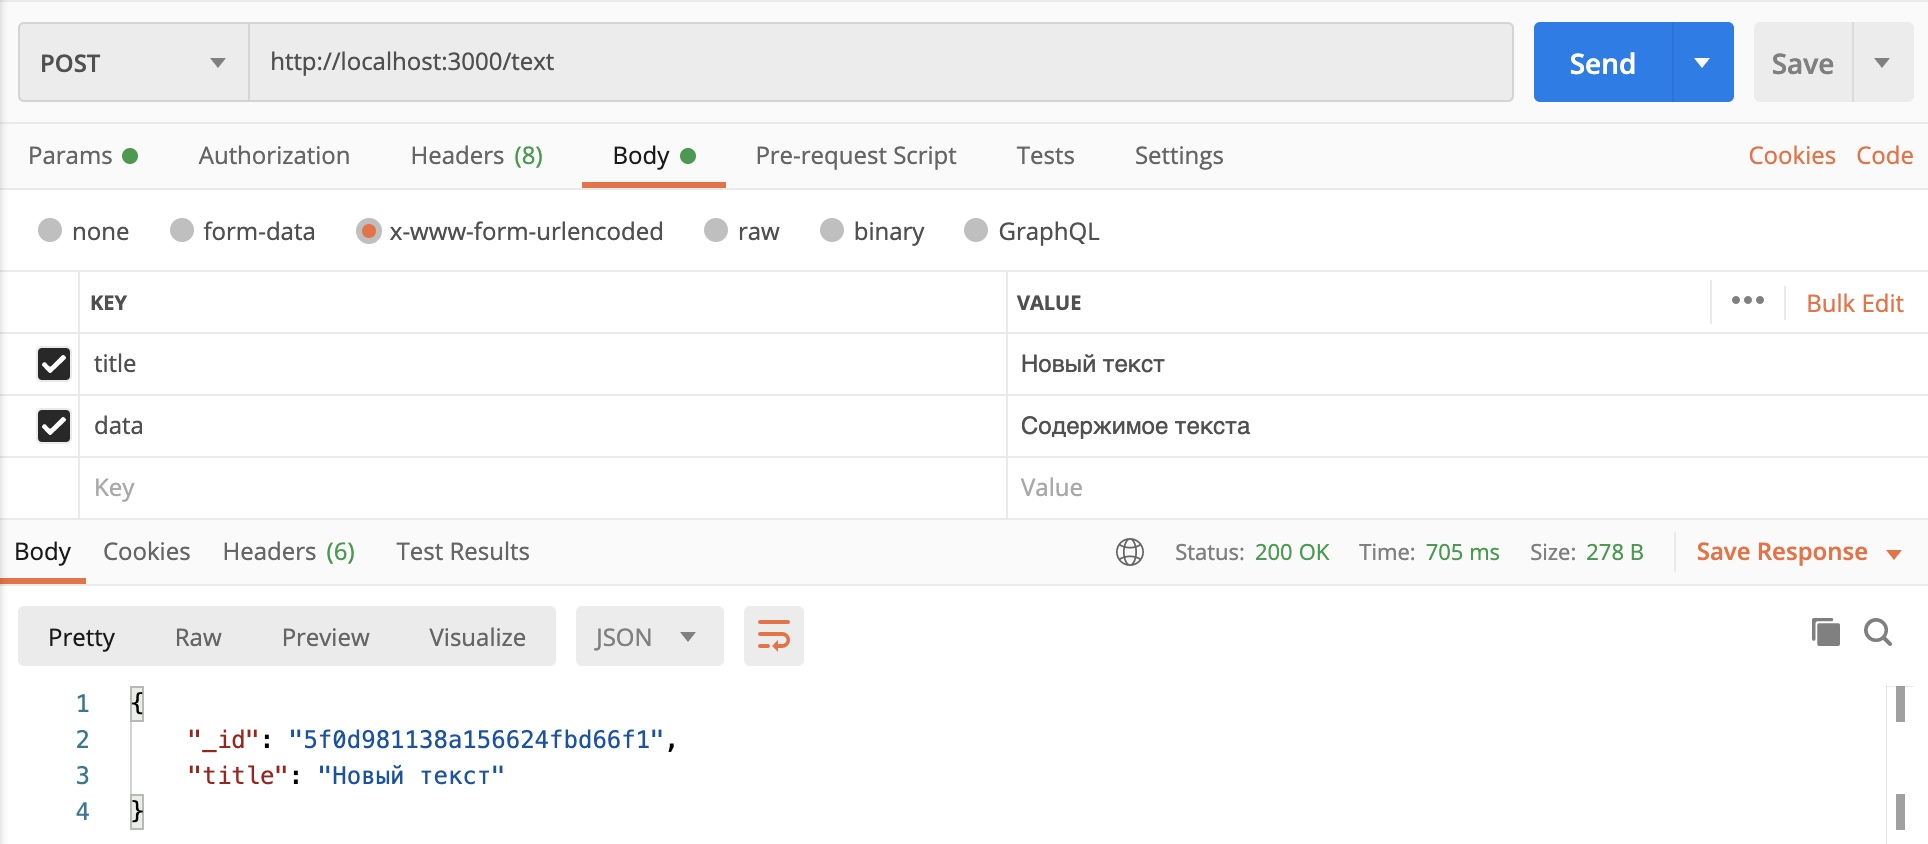
\includegraphics[scale=0.25]{2}

Отправим post запрос с телом title:test и каким то текстом в data. Судя по описанию api приложение должно вернуть мне структуру с id нового обьекта, а также его title. Что и отображается ниже в body, правее указывается код операции - 200, запрос прошел успешно, также вес письма и время выполнения.

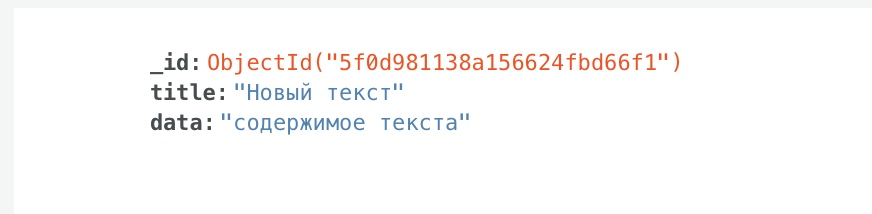
\includegraphics[scale=0.25]{3}

Если мы зайдем на mLab в коллекцию text, мы увидем новый обьект с id, который совпал с вернувшейся id в структуре.

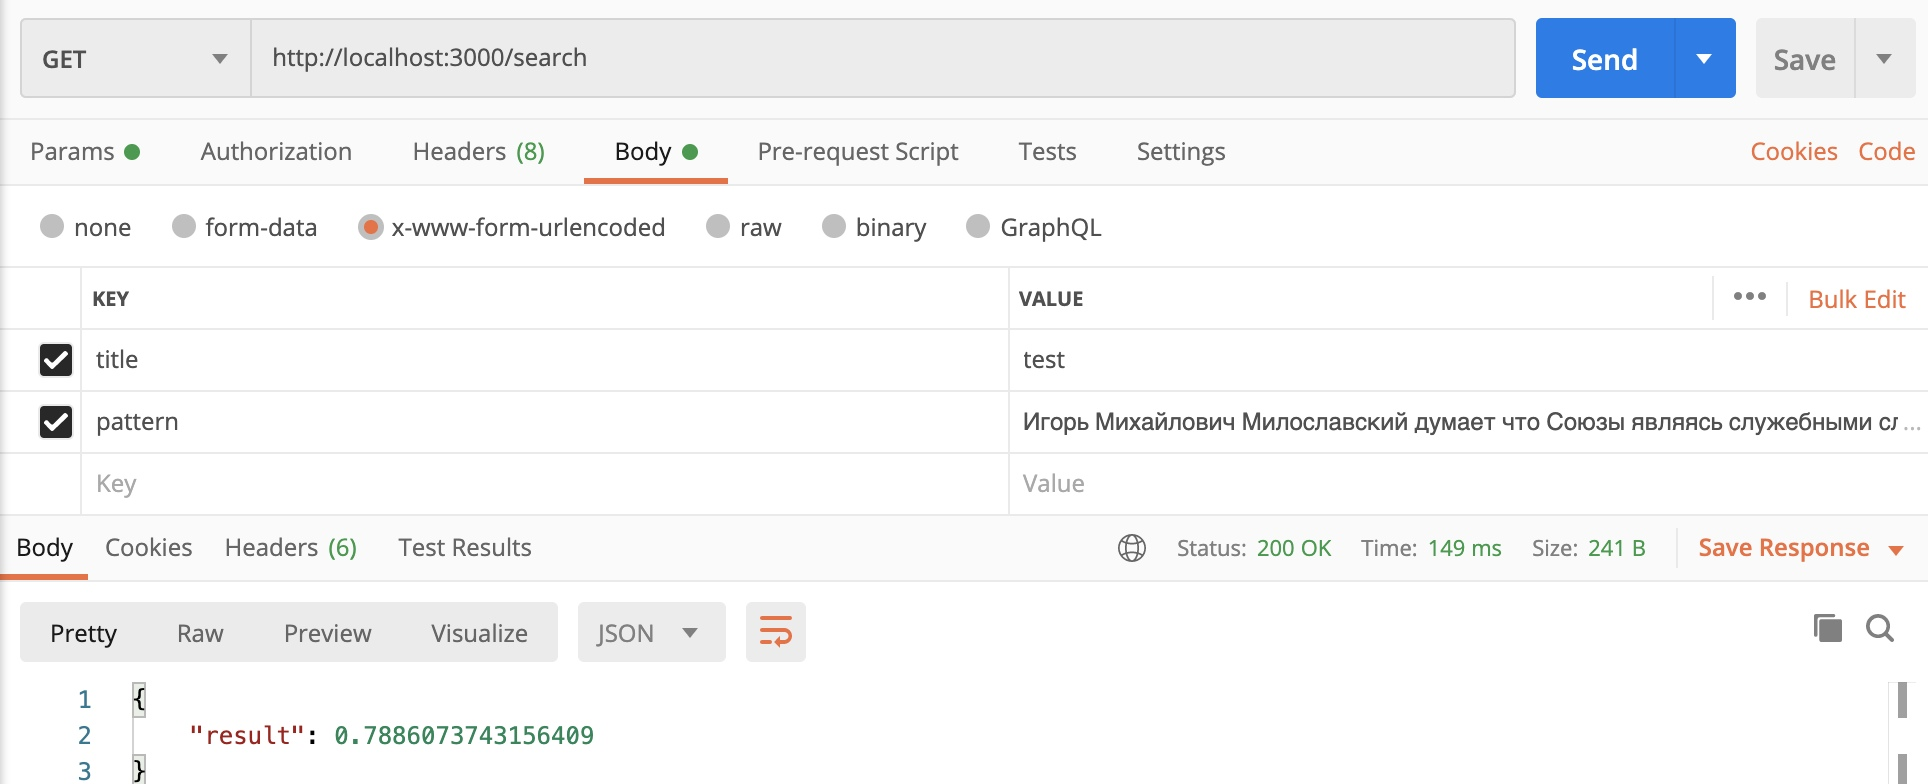
\includegraphics[scale=0.25]{1}

В примере выше мы отправили get запрос на url localhost:3000/search с атрибутами title и pattern, что же делает в этом случае сервер?

\begin{lstlisting}[language=JavaScript]
app.get('/search', (req, res, next) => {
    if (!req.body.title) {
        next();
    } else {
        const details = {title: req.body.title};
        db.collection('text').findOne(details, (err, item) => {
            if (err) {
                res.send({ 'error': 'An error has occured' });
            } else {
                var re = Shingl(req.body.pattern.toLowerCase(), item.data);
                res.send({ result: re });
            }
        });
    }
});
\end{lstlisting}

Приложение регестрирует url /search, так как функция обработки является асинхронной, вызывать код последовательно бесполезно, поэтому используем callback с параметрами req (тело запроса), res(тело ответа) и next(следующий middleware, если текущий не сможет обработать запрос).

Делается запрос к базе данных по нужному фильтру, ответ уходит в callback, на основании ответа формируется ответ, либо ответ процента плагиата, либо код и тело ошибки.

На фотографии Postman мы видим ответ, в разделе body, вернул нам структуру с result равным 0.78.




\section*{Ссылка на GitHub}

https://github.com/pagamov/4sem/tree/master/summer\%20task

\pagebreak

\end{document}

